\documentclass{article}
\usepackage{graphicx} % Required for inserting images
\usepackage{float}
\usepackage{booktabs} % For better horizontal lines

\usepackage[T1]{fontenc}
% \title{Analysing the Robustness of Deep Neural Networks}
% \author{Divij Khaitan}
% \date{\today}
\usepackage{longtable}
\usepackage{amsmath}
\usepackage{amssymb}
\usepackage{subcaption}
\DeclareMathOperator{\softmax}{softmax}
\begin{document}

    % \maketitle

    \begin{titlepage}
        \centering
        \vspace*{1in}
        {\Huge\bfseries Capstone Project - Deep Learning Study \par}
        \vspace{1.5in}
        {\Large\itshape Divij Khaitan \par}
        \vspace{1.5in}
        {\large\itshape Supervisor: Subhashis Banerjee \par}
        \vfill
        {\large \today\par}
    \end{titlepage}
    \pagenumbering{roman} % Roman numerals for preliminary pages
    \tableofcontents
    \clearpage

    % Main Content
    \pagenumbering{arabic} % Switch to Arabic numerals
    \section{Introduction}
        The goal of this project is to introduce a new framework for the analysis of the robustness properties of deep neural networks by analysing the patterns of neuron activations. A shortcoming of the existing work on out-of-distribution detection is that the notions of training and test distributions are very loosely defined in literature, and isn't clear if they can be well defined at all. However, the values taken on by the neurons and circuits in a neural network can be used to define a distribution. The goals of this framework are
        \begin{enumerate}
            \item 
                Defining data distributions with regards to a trained network as opposed to a training dataset
            \item 
                Provide a diagnostic tool to detect when a network has overfit with polynomial overhead over the training process
            \item 
                To detect distribution shifts on same-task transfer learning before deployment
        \end{enumerate}
        Our contributions are as follows 
        \begin{itemize}
                \item 
                    Providing a framework to assess the robustness of a trained neural network in a more principled manner than checking accuracy or perturbations that may never naturally occur.
                \item 
                    Extracting distributions from trained networks to address the problem of distribution shifts in a principled manner 
                \item 
                    Developing a method for checking distances between datasets at deployment-time
            \end{itemize}

        \subsection{Related work}
            \indent \textbf{Generalisation/Implicit Regularisation}: Zhang et. al. showed as early as 2017 that even AlexNet has enough capacity to fit all of imagenet with completely random labels perfectly when given enough time \cite{zhang2017understandingdeeplearningrequires}. This suggests that although networks have extremely high 'capacity', they do not use all of it in practice and that contrary to statistical wisdom, they are not overfitting as a result of overparameterisation. Arora et. al. showed that overparameterisation provides a speed up to the optimisation of neural networks and provided bounds for the generalisation error of two layer ReLU networks \cite{pmlr-v80-arora18a}. Soltanolkotabi and Oymak showed that networks that polynomially overparameterised in the size of the input are resistant to label corrpution, with the final parameters being close to their initialised values \cite{pmlr-v108-li20j}. A major hypothesis in this area is that stochastic gradient descent (SGD) as a training method introduces an 'implicit regularisation' into the training of a deep network. Norm minimisation was one explanation for this behaviour, first put forth by \cite{neyshabur2015searchrealinductivebias}. Several notions of complexity have been put forth, including VC dimension and Rademacher complexity, see \cite{neyshabur2017implicitregularizationdeeplearning} for a more granular view of these. Examples where all matrix norms diverge were constructed in \cite{razin2020implicitregularizationdeeplearning}, indicating that the relationship between weight decay and implicit regularisation requires more inspection. This relationship has also been questioned by \cite{arora2019implicitregularizationdeepmatrix}, which shows that for the case of matrix factorisation, matrix norms are insufficient to describe the action of gradient-based optimisation. This paper also shows that adding depth to matrix factorisation encourages low rank solutions, which improve the accuracy of the reconstruction. \cite{gissin2019implicitbiasdepthincremental} formally showed that deep networks learn 'incrementally', and while shallow networks can exhibit similar behaviour they do so for a small set of initial conditions. \cite{arpit2017closerlookmemorizationdeep} showed that SGD behaves differently on noise as opposed to actual datasets, and that dropout works better than noise injection for hindering memorisation while promoting generalisation

            \textbf{Out of Distribution Detection}: When considering open world deployment of networks, it simply isn't possible to train them on exhaustive partition of every input they can expect. Thus, it becomes important to develop mechanisms that allow users to detect when an input is outside the training distribution of a model. The first major work that tackled this problem with some effectiveness was \cite{hendrycks2018baselinedetectingmisclassifiedoutofdistribution}, which uses $-\max_i \softmax(f(x)_i)$ as a means of detecting if a particular input is outside the training distribution. This is analogous to treating the magnitude of the softmax output as a confidence measure, which isn't entirely accurate as pointed out by the authors. However, this has proven to be a baseline which is difficult to beat non-trivially. \cite{hendrycks2019deepanomalydetectionoutlier} describes a method for fine-tuning trained models to detect OOD inputs using unlabelled data and the KL divergence from a uniform distribution. ODIN \cite{liang2020enhancingreliabilityoutofdistributionimage} has empirically shown excellent performance on OOD detection, but requires tuning hyperparameters beforehand. \cite{lee2018simpleunifiedframeworkdetecting} Uses a similar idea of creating a probability distribution over feature spaces and uses the minimum mahalanobis distance as a classifier, and also use it to show that tuning their classifier on certain adversarial attacks adds robustness to other adversarial attacks. The authors assume a multivariate gaussian distribution on the class-conditional softmax probability vectors, and for a vector output the class for which the probability vector has the smallest mahalanobis distance. All of these fall into the class of post-hoc OOD detection methods, which includes \cite{liu2021energybasedoutofdistributiondetection, sun2022diceleveragingsparsificationoutofdistribution, morteza2021provableguaranteesunderstandingoutofdistribution}. Another line of thought introduced in \cite{sun2021reactoutofdistributiondetectionrectified} suggests that large activation values are caused by improper normalisation and that activation clipping separates the in and out of distribution data is also explored by \cite{ahn2023lineoutofdistributiondetectionleveraging} when combining it with a significance measure based on shapely values.
            % TODO: Concept and Covariate Shift, add and explain literature
            
            \textbf{Interpretability}: There has been some past work on analysing the patterns of activation of neural networks. On the side of interpretability, SUMMIT \cite{hohman2019summitscalingdeeplearning} and NAP \cite{bauerle2022neuralactivationpatternsnaps} both attempt to identify important neurons in an attempt to interpret the features associated with different classes. \cite{stano2020explainingpredictionsdeepneural} fits a mixture of gaussians to each neuron independently in selected layers with the explicit goal of attributing predictions to neurons. They use at most 2 gaussians. Similar ideas have been used for the detection of rare classes \cite{paterson2021detectionmitigationraresubclasses} as well as the detection of out-of-distribution inputs \cite{olber2023detectionoutofdistributionsamplesusing}. \cite{simonyan2014deepinsideconvolutionalnetworks, faaaf4beb6f24ca599a7ecae54e0c724, Selvaraju_2019, gautam2021lookslikethatenhancing} focus on mapping each input pixel to an importance value, while \cite{ribeiro2016whyitrustyou, lundberg2017unifiedapproachinterpretingmodel} focus on importance of each feature locally around a particular datapoint. \cite{gautam2024prototypicalselfexplainablemodelsretraining} uses clustering in the embedding space alongside PRP \cite{gautam2021lookslikethatenhancing} characterise the prediction of any model in terms of it's similarity to a set of prototypes - images which are representative of the rest of the class - which is obtained by clustering embeddings in the latent space.
            
            \textbf{Mechanistic Interpretability and Superposition of Neurons}: Mechanistic Interpretability particularly aims to 'reverse engineer' a neural network by connecting parts of a network to semantic concepts that can be understood by humans. \cite{olah2017feature} uses optimization to backpropogate the activations for particular neurons to see which portions of images they are most sensitive to. They find that high frequency patterns are a common occurence when following the path of steepest descent, and this leads to pathological examples that the network will never actually see. The conclusion of the work is that this can be fixed by penalising high frequency patterns. A follow-up paper in 2018 focuses on the interaction between different parts of the network, as well as creating interfaces to make sense of these interaction at a human scale \cite{olah2018the}. \cite{olah2020zoom} claims that alongside the neurons, it is also the connections between them that hold semantic meaning and can be studied. Empirical evidence from InceptionV1 shows that curve detecting convolutional filters in early layers directly inhibit and activate parts of filters that detect more complicated shapes in later layers. Additionally, they find that a single monosemantic neuron detecting cars in one layer spreads the feature over multiple neurons in the next layer that seem to be detecting dog faces. This phenomenon is called superposition, and is studied empirically over the course of several papers \cite{elhage2022solu, elhage2022superposition, bricken2023monosemanticity, templeton2024scaling, lindsey2025biology} particularly for LLMs. The idea behind superposition is that concepts are encoded as directions in a latent space, and when the concepts are sparse and more numerous than the dimensionality of the latent space, the network encodes them as into non-orthogonal directions. A consequence of this is that neurons are polysemantic and activate for multiple concepts as well as the fact that the neurons themselves need not be the unit of interpretation.  

            \textbf{Adversarial Robustness}: Szegdy et. al. discovered \cite{szegedy2014intriguingpropertiesneuralnetworks} in 2014 that classifiers on vision models are susceptible to extremely small changes (in some $L^p$ space) that can cause a misclassfification. Since then, a considerable amount of work has gone into attempting to explain their existence (\cite{shafahi2020adversarialexamplesinevitable}, \cite{shamir2022dimpledmanifoldmodeladversarial}) and the development of attacks (PGD \cite{madry2019deeplearningmodelsresistant}, FGSM\cite{goodfellow2015explainingharnessingadversarialexamples}) and defenses to those attacks, either by changing the loss function or by modifying the training algorithm in some way. 
            
            \textbf{Manifold Hypothesis}: This is an idea that pre-dates deep learning, that most real-world datasets in high dimensions have an underlying low dimensional structure. In the context of machine learning, it has primarily been studied from the perspective of dimensionality reduction, reducing a set of points in a high dimensional space to one in a low dimensiona space which is equivalent to it. \cite{fefferman2013testingmanifoldhypothesis} develops an algorithm to test the hypothesis, and \cite{NIPS2010_8a1e808b} discusses the sample complexity of the problem. See \cite{meil2023manifoldlearningwhathow} for a survey of the most recent methods in the field. 

            % \textbf{Lottery Ticket Hypothesis}: The sparsity of activations in neural networks is widely seen in practice. Frankle and Carbin suggested that a small subset of neurons are better primed to fit the dataset at initialisation time, and dubbed this the 'lottery ticket hypothesis'. Subsequent work has focused on algorithms for identifying such lottery tickets. 
    \section{Methods}
        % Shifts in distribution are situation when the distributions of the training and testing sets are not identical. In literature, the most common classification of these shifts are concept shift and covariate/data shift.

        % \textbf{Covariate Shift} is when $p(x)$ changes, but not $p(y|x)$, i.e. the inputs change but the labels stay the same. An example would include training a model on voting patterns for India, and testing the model on voting patterns from China.
        
        % \textbf{Concept Shift} is when $p(x)$ remains the same, but $p(y | x)$ does not. This can be thought of as training on a similar dataset with slightly different labels. An example would be training a model to issue red alerts for storms in Delhi, and testing it to issue red alerts in Pune. While both cities might see similar rainfall patterns, they may be equipped very differently to handle the same amount of precipitation. 

        % Detecting such shifts can be difficult in practice, because the distributions themselves cannot be characterised easily. Our hypothesis is that in CNNs, the neurons from the fully connected layers should have similar activation patterns across the same classes, and thus we should be able to attach distributions of neuron activations to each class, which should be sensitive to a shift in the distribution of inputs. 
        
    % \section{Class-wise Frequencies of Neuron Activations}
    %     For this section, we analysed the outputs of each fully connected hidden layer, i.e. for a network $f = \phi_{n}(f_{n}(\dots(\phi(f_1(x)))))$, we analysed $x_k = \phi(f_{k}(\dots(\phi(f_1(x)))))$. Alexnet in particular is RELU-activated with the exception of the final layer, so $\phi_i = \text{ReLU} \text{ if } i < n \; \sigma(x) \text{ if } i = n$. We utilised the following definitions of significance \\
    %     \[S_1(x_{i}) = 1 \text{ if } x_i > 0\] 
    %     \[S_2(x_{(i)}) = 1 \text{ if } \frac{x_{(i)}}{x_{i+1}} > \epsilon\] 
    %     $x_{(i)}$ denotes the i$^\text{th}$ order statistic. The first definition is comes from the ReLU activation, where a neuron is considered 'active' if it is positive. The justification for the second is the assumption of a high signal to noise ratio, where smaller activations correspond to noise while larger activations correspond to meaningful information. Practically, we set the value of $\epsilon$ to be 1000. We computed the proportions of every neuron activating in any given class under both definition, and the results are attached below. Each neuron has a proportion of activations for each class in between 0 and 1, we have displayed histograms of the number of neurons in 100 bins for different activation proportions. Below is the result for a particular class under both $S_1$ and $S_2$. The y-axis is the number of neurons in each bin, and the x-axis has the bins of different proportions of activation across all the images in the class. This shows a move towards sparsity in activation with an increase in depth.
    %     \begin{figure}[H]
    %         \centering
    %         \begin{minipage}{0.45\textwidth}
    %             \centering
    %             \includegraphics[width=\textwidth]{images/alexnet_class_frequenn01601694.png}
                
    %         \end{minipage}\hfill
    %         \begin{minipage}{0.45\textwidth}
    %             \centering
    %             \includegraphics[width=\textwidth]{images/alexnet_class_frequenthreshold_n01601694.png}
    %         \end{minipage}
    %         \caption{Histograms for AlexNet activations under $S_1$(left) and $S_2$(right). There is a distinct clustering towards the left inside the convolutional layers (plots 1 to 5) and then inside the fully connected layers as well (plots 6 and 7)}
    %         \label{fig:neuron_activation_frequency}
    %     \end{figure}

    %     % \begin{figure}[ht]
    %     %     \centering
    %     %     \includegraphics[height=\textheight,keepaspectratio]{vgg11_bn_class_frequenn01601694.png}
    %     %     \caption{Histogram for VGG11 with thresholding. We observe the same behaviour here}
    %     %     \label{fig2}
    %     % \end{figure}
    % \section{Class-wise Patterns of Neuron Activations}
    %     We also plotted the proportion of successes of each neuron in each layer. Some of the results for the final layer of different classes are attached below. The key takeaway is once again the sparsity of the activations, with most neurons having small activations and a few neurons having large activations. For ease of viewing, the vectors were ravelled to form a rectangle with approximately equal sides. Below attached are results from the final 2 layers of a single class.
    %     \begin{figure}[H]
    %         \centering
    %         \begin{minipage}{0.45\textwidth}
    %             \centering
    %             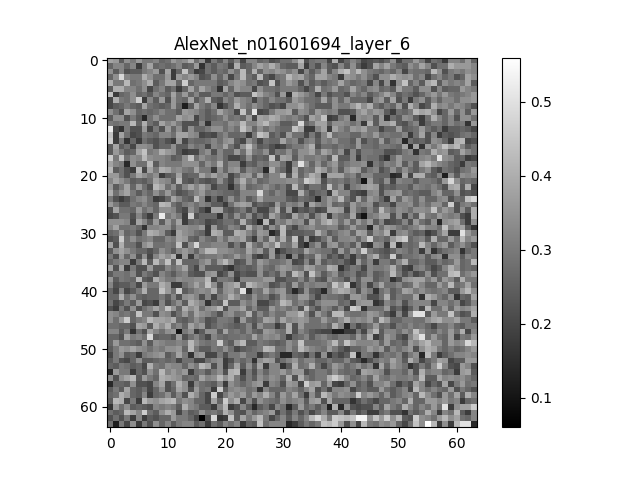
\includegraphics[width=\textwidth]{images/AlexNet_n01601694_layer_6.png}
                
    %         \end{minipage}\hfill
    %         \begin{minipage}{0.45\textwidth}
    %             \centering
    %             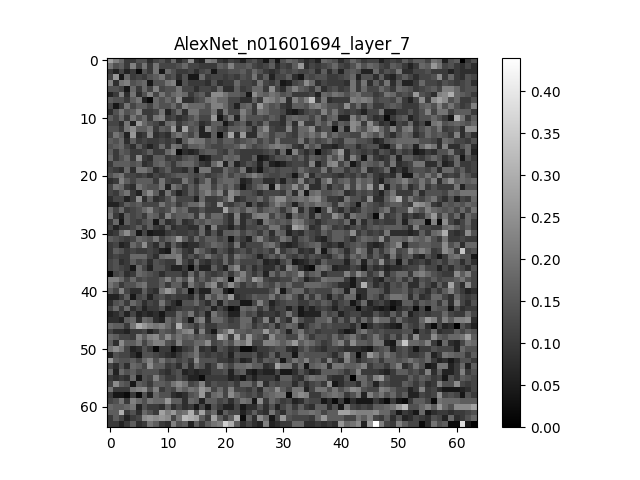
\includegraphics[width=\textwidth]{images/AlexNet_n01601694_layer_7.png}
    %         \end{minipage}
    %         \caption{Activation proportions of neurons for the fully connected layers 6 and 7 of alexnet}
    %         \label{fig:neuron_activation_pattern}
    %     \end{figure}
        
    % \section{Entropies in Between Classes}
        
        \subsection{Class-Wise Frequencies of Significant Paths Interactions}
            The focus of the study was the interactions of neurons and weights together. Thus, instead of just looking at the final value of the neuron, we decided to look each circuit that extends across a single layer and corresponds to a single pair of neuron and weight. In this case, what we did is described below. 

            The final layer of the neural network operates as follows. Given an activation vector $x \in \mathbb{R}^{n_{in} \times 1}$ and a weight matrix $W \in \mathbb{R}^{n_{out} \times n_{in}}$. The 3 interpretations we study here are
            \begin{itemize}
                \item 
                    Fitting a bernoulli random variable to each path after binarising: This is discussed below. A significant downside is the correlations neurons firing together is lost
                \item 
                    Fitting a multivariate gaussian to the raw path values: This will be discussed in a later section. While this captures both path information and covariance, it may become computationally infeasible due to large memory requirements
                \item 
                    Fitting a multivariate gaussian to the neurons: This will be discussed in a later section. This loses path information for a more granular modelling of neuron activations. 
            \end{itemize}
                \[
                    \begin{bmatrix}
                        w_{1,1} & \dots & w_{1,n_{in}} \\
                        \vdots & \ddots & \vdots \\
                        w_{n_{out}, 1} & \cdots & w_{n_{out}, n_{in}} \\
                    \end{bmatrix}
                    \begin{bmatrix}
                        x_1 \\
                        \vdots \\
                        x_{n_{in}} \\
                    \end{bmatrix}
                    = 
                    \begin{bmatrix}
                        w_{1,1}x_1 + w_{1, 2}x_2 + \dots + w_{1, n_{in}}x_{n_{in}} \\
                        \vdots \\
                        w_{n_{out},1}x_1 + w_{n_{out}, 2}x_2 + \dots + w_{n_{out}, n_{in}}x_{n_{in}}
                    \end{bmatrix}
                \]
                This would not allow us to study the individual activation-weight pairs, because they would all be summed up. A vector operation that computes the sum over the rows of a matrix is postmultiplication by the all 1s vector, so by factoring out this vector we can get the required information. Factoring out the all 1s vector from the neurons in the penultimate layer, we get an diagonal matrix with the neurons activations as entries 
                \[
                    \begin{bmatrix}
                        w_{1,1} & \dots & w_{1,n_{in}} \\
                        \vdots & \ddots & \vdots \\
                        w_{n_{out}, 1} & \cdots & w_{n_{out}, n_{in}} \\
                    \end{bmatrix}
                    \begin{bmatrix}
                        x_1  & \dots & 0 \\
                        \vdots & \ddots & \vdots \\
                        0 & \dots & x_{n_{in}} \\
                    \end{bmatrix}
                    = 
                    \begin{bmatrix}
                        w_{1,1}x_1  & \dots & w_{1,n_{in}}x_1 \\
                        \vdots & \ddots & \vdots \\
                        w_{n_{out}, 1}x_{n_{in}} & \dots & w_{n_{out}, n_{in}}x_{n_{in}} 
                    \end{bmatrix}\]
            To this, we concatenated the bias vector as an additional neuron, giving us a matrix in $\mathbb{R}^{n_{out} \times (n_{in} + 1)}$. The distribution fitting was done after flattening the matrix into a vector of dimension $\mathbb{R}^{1 \times (n_{out}(n_{in} + 1))}$. 
            \[\begin{bmatrix}
                    w_{1,1}x_1 \\
                    \vdots \\
                    w_{1,n_{in}}x_{n_{in}} \\
                    \vdots \\
                    w_{n_{out},1}x_{1} \\
                    \vdots \\
                    w_{n_{out}, n_{in}}x_{n_{in}} \\
                    \vdots
                    b_1 \\
                    \vdots \\
                    b_{n_{out}}
                \end{bmatrix}\]
            The definition of significance used was 
            \[S(x_{ij}) = 1 \text{ if } |x_{ij}| > \frac{|\sum_j x_{ij}|}{n_{in}} \]
            where $n_{in}$ is the number of input features, i.e. number of columns in the matrix. The justification behind this is the idea that if an activation has an above average contribution to the final activation, the path is significant.
            As eariler, we hypothesise that the number of significant interactions between neurons and weights are sparse, and that the sparsity increases with depth. 
            
        \subsection{KL Divergence Between Classes}
            Building on the same experiment, we wanted to check both the entropies in between different classes over the activation distribution for the same layer. We also measured the same entropies at training and testing time, as well as an in and out of distribution dataset. The in-distribution dataset was the validation set for imagenet as used eariler, and the out of distribution dataset was the imagenet-r dataset created by Hendrycks et. al.\cite{hendrycks2021facesrobustnesscriticalanalysis}. This is a collection of stylised versions of the standard classes of imagenet such as caricatures. This dataset has 200 classes compared to the original 1000 from imagenet, and to ensure the comparison was meaningful we sampled 50 classes from the dataset uniformly at random and computed the pairwise KL divergences between pairs of classes from the imagenet validation set, between pairs of classes from the imagenet-r set and between the same classes from imagenet and imagenet-r. Along similar lines, we also measured the entropy of the distributions. Analagous to regression, the distance within the clusters (entropy) should decrease, while the distance between the clusters (KL divergence) should increase. The entropy is given by the formula
            \[H(X) = -\sum p(x)\log(p(x))\]
            Where $p(x)$ is the probability that the random variable $X$ takes on the value $X$. Intuitively, it is a measure of 'disorder' in the random variable. The KL divergence is the relative entropy between 2 distributions, given by the formula 
            \[D_{KL}(P||Q) = \sum P(x)\log(\frac{P(x)}{Q(x)})\]
            This can be thought of as a measure of how well $P$ approximates $Q$. It is not a true metric, because it doesn't satisfy triangle inequality or symmetry. Our computations make a strong assumption of \textbf{independence} of the significance of activations, i.e. that any activation will be significant in it's own row is independent of the other events being significant. 
            An idea the framework pushes is probabilistic interpretation of class separation. To compare, we flatten the proportion matrices to vectors in $\mathbb{R}^{n_{in}\times n_{out}}$ and compute the euclidean distance between them, which is a geometric quantity. 
        
        \subsection{Log Probabilities for Distribution Shift Detection}
            Given that we have a distribution over different datasets, a natural question to ask is if they register different behaviour for in-distribution and out-of-distribution data. For this, only the CIFAR10 dataset was used, with CIFAR10.1 \cite{recht2018cifar10classifiersgeneralizecifar10} providing a frame-of-reference dataset which was meant to be similar and TinyImagenet \cite{Le2015TinyIV} and SVHN \cite{37648} used as OOD datasets. Since separation between individual classes cannot be tracked because of label incoherence, the comparison is made across the distribution aggregated over the entire dataset. Alongside this, we measure 
            \begin{itemize}
                \item 
                    The separation of datasets at an aggregate level
                \item 
                    The posterior probability of having observed an activation of an image $x$ given that it comes from a dataset $Y$, i.e. $p(f(x)| x \sim Y)$ across the different dataset choices $Y$. Y here is a multivariate bernoulli distribution. Separation of different datasets under this score would make this a good metric for distribution shift detection. 
            \end{itemize}
            The sampled classes from imagenet are quite semantically varied, containing classes from cellular telephone to labrador retriver. A full list is provided in Appendix D. Imagenet-R on the other hand, contains stylised versions of the same classes sampled from Imagenet such as caricatures. CIFAR10 too has some animal classes like frog and deer and some vehicle classes such as truck or automobile which are quite varied. Tiny Imagenet needs to have a mapping to CIFAR10 crafted by hand. The mapping decided by us can be found in Appendix A. On the other hand, SVHN comes from a completely different domain. It contains images of numberplates from houses all across the world, which are vastly different from natural images of animals or vehicles. 
        
        \subsection{Modelling Activations using a Multivariate Gaussian}
            The matrix of paths for each image can flattened
            \[\begin{bmatrix}
                w_{1,1}x_1  & \dots & w_{1,n_{in}}x_1 \\
                \vdots & \ddots & \vdots \\
                w_{n_{out}, 1}x_{n_{in}} & \dots & w_{n_{out}, n_{in}}x_{n_{in}} 
            \end{bmatrix} 
            \rightarrow 
            \begin{bmatrix}
                w_{1,1}x_1 \\
                \vdots \\
                w_{1,n_{in}}x_{n_{in}} \\
                \vdots \\
                w_{n_{out},1}x_{1} \\
                \vdots \\
                w_{n_{out}, n_{in}}x_{n_{in}} \\
            \end{bmatrix} = X
            \]
            The following estimators can be used for the mean and variance of the distribution. Note that this assumes the distribution is gaussian, because it is being modelled entirely using just the mean and variance. Given images $x_1, \dots, x_n$ for a class $c$, it's mean and covariance can be estimated as
            \[\vec{\mu_c} = \frac{1}{n}\sum_{i=1}^n \vec{x}_i\]
            \[\Sigma_c = \frac{1}{n}\sum_{i=1}^n (\vec{x}_i - \vec{\mu_c})(\vec{x}_i - \vec{\mu_c})^T\]
            \[d_{\text{mahalanobis}}(c_1, c_2) = \sqrt{((\vec{\mu_{c_1}} - \vec{\mu_{c_2}})^T\Sigma_{c_1}(\vec{\mu_{c_1}} -\vec{\mu_{c_2}}))}\]
            This was done at the path level as explained above, as well as the neuron level. The justification for doing it at the neuron level is that with regards to a fixed network, looking at the paths may not always be necessary and is much more resource intensive. To specify, the mean and variances are estimated in the same way with the only change being
            \[X = 
            \begin{bmatrix}
                x_1 \\
                \vdots \\
                x_{n_{in}} \\
            \end{bmatrix}
            \]
            To avoid issues with numerical stability, a low rank approximation of the covariance matrix was used, with small imaginary components being ignored. In addition to the flattened products of neurons and weights, this is also applied to the neurons themselves. 
        
        \subsection{Memorisation and Significance}
            We hypothesise that a network which has memorised it's training data would have significantly different properties in terms of sparsity and the separation of classes. To this end, we replicate the experiment specified in \cite{zhang2017understandingdeeplearningrequires} and train a modified version of AlexNet on CIFAR10 until it reaches zero error. The details of the training stay the same and will be provided in Appendix B. 
        
        \subsection{Adversarial Attacks}
            The above gives us a distribution on the activations for a given class. We compared the probabilities conditioned on the distribution of the class of the validation images subject when subjected to a PGD attack \cite{madry2019deeplearningmodelsresistant}. The parameters of the attack are given in Appendix C. 
        
        \subsection{Manifold Entaglement}
            In the final hidden layer, the low-dimensional manifolds for different classes should be linearly separable. This is because the remaining transformations the network will apply are an affine hidden layer computation and a linear softmax computation. We estimate the dimensionality of the manifolds spanned by each class by inspecting the neurons for this layer, combining them into a matrix and finding it's rank. We further estimate the degree of overlap between the manifolds by combining the matrices for different classes and then applying the principle of inclusion and exclusion. Networks that have not overfit their training data should have manifolds with little overlap, while those which have should have entagled class manifolds. We additionally expect the manifolds to have smaller dimensionality for networks with better embeddings. 

    \section{Results}
        We examined the distributions for AlexNet, VGG, ResNet and InceptionV3. The experiments were run using PyTorch, and the weights for the pretrained versions of the networks were also taken from there. The datasets used were the validation sets for Imagenet \cite{russakovsky2015imagenetlargescalevisual}, and CIFAR10 \cite{Krizhevsky2009LearningML}
        \subsection{Modelling Significant Activations as Bernoulli Distributions}
            
            \subsubsection{Sparsity of Activations}
                The following plots have the number of times a neuron activated over the entire validation set divided by the length of the validation set on the x axis, and the y-axis is the number of neurons that activate in that 'bin', divided by the total number of neurons.
                The results indicate that training encourages sparsity quite strongly, with the proportions of neurons that are always on dropping from 0.2 and 0.1 to 0.05 and $<$ 0.01 on the last and second last layers respectively from the untrained model to the best model. The network fitting random labels has an extremely sparse penultimate layer, with the best network having some density to it and the overtrained network resembling a mid-point in between the random labelled and the best network. 
                
                \begin{figure}[H]
                    \centering
                    \begin{minipage}{0.45\textwidth}
                        \centering
                        \includegraphics[width=\linewidth]{new/small_alexnet_untrained_cifar10/activation_proportions/0.png}
                        \subcaption{Untrained}
                        % \label{fig:image1}
                    \end{minipage}
                    \hfill
                    \begin{minipage}{0.45\textwidth}
                        \centering
                        \includegraphics[width=\linewidth]{new/small_alexnet_cifar10_random_labels/activation_proportions/0.png}
                        \subcaption{Random Labels}
                        % \label{fig:image2}
                    \end{minipage}
                    \begin{minipage}{0.45\textwidth}
                        \centering
                        \includegraphics[width=\linewidth]{new/small_alexnet_cifar10_250_epoch/activation_proportions/0.png}
                        \subcaption{Overtrained}
                        % \label{fig:image1}
                    \end{minipage}
                    \hfill
                    \begin{minipage}{0.45\textwidth}
                        \centering
                        \includegraphics[width=\linewidth]{new/small_alexnet_cifar10_best/activation_proportions/0.png}
                        \subcaption{Best}
                        % \label{fig:image2}
                    \end{minipage}
                    \hfill
                    
                    \caption{Activation Proportions from the class Airplane on the last and second last layers on different versions of the Modified AlexNet}
                    \label{fig:class_airplane}
                \end{figure}
                
                \begin{figure}[H]
                    \centering
                    \begin{minipage}{0.45\textwidth}
                        \centering
                        \includegraphics[width=\linewidth]{new/small_alexnet_untrained_cifar10/activation_proportions/7.png}
                        \subcaption{Untrained}
                        % \label{fig:image1}
                    \end{minipage}
                    \hfill
                    \begin{minipage}{0.45\textwidth}
                        \centering
                        \includegraphics[width=\linewidth]{new/small_alexnet_cifar10_random_labels/activation_proportions/7.png}
                        \subcaption{Random Labels}
                        % \label{fig:image2}
                    \end{minipage}
                    \begin{minipage}{0.45\textwidth}
                        \centering
                        \includegraphics[width=\linewidth]{new/small_alexnet_cifar10_250_epoch/activation_proportions/7.png}
                        \subcaption{Overtrained}
                        % \label{fig:image1}
                    \end{minipage}
                    \hfill
                    \begin{minipage}{0.45\textwidth}
                        \centering
                        \includegraphics[width=\linewidth]{new/small_alexnet_cifar10_best/activation_proportions/7.png}
                        \subcaption{Best}
                        % \label{fig:image2}
                    \end{minipage}
                    \hfill
                    
                    \caption{Activation Proportions from the class Frog on the last and second last layers on different versions of the Modified AlexNet}
                    \label{fig:class_frog}
                \end{figure}
                The proportion histograms for the last 3 layers of alexnet on imagenet and imagenet-r are in figure \ref{fig:frequency_neuron_weight1}. For AlexNet, we can see that the randomly initialised network looks the same in terms of activation proportions for all the layers across both datasets. We once again see that training encourages sparsity in the network, even on the out of distribution set. The in-distribution dataset is sparser on the final layer and the penultimate layers. In fact, there is a significant increase in the proportion of stray activations on the out of distribution dataset, suggesting that sparsity may be a characteristic of learning. 
                \begin{figure}[H]
                    \centering
                    \begin{minipage}{\textwidth}
                        \centering
                        \includegraphics[width=\textwidth]{new/alexnet_untrained_imgr_out/activation_proportions/n02088466.png}
                        
                    \end{minipage}\hfill
                    \begin{minipage}{\textwidth}
                        \centering
                        \includegraphics[width=\textwidth]{new/alexnet_imgr_out/activation_proportions/n02088466.png}
                    \end{minipage}
                    \begin{minipage}{\textwidth}
                        \centering
                        \includegraphics[width=\textwidth]{new/alexnet_untrained_r/activation_proportions/n02088466.png}
                        
                    \end{minipage}\hfill
                    \begin{minipage}{\textwidth}
                        \centering
                        \includegraphics[width=\textwidth]{new/alexnet_r/activation_proportions/n02088466.png}
                    \end{minipage}
                    
                    \caption{Frequencies of the significant paths activation proportions for the networks: untrained on imagenet, trained on imagenet, untrained on imagenet-r and  trained on imagenet-r from top to bottom}
                    \label{fig:frequency_neuron_weight1}
                \end{figure}
                
                % \begin{figure}[H]
                %     \centering
                %     \begin{minipage}{\textwidth}
                %         \centering
                %         
\includegraphics[width=\textwidth]{new/alexnet_/alexnet_untrained_imgr_n01443537.png}
                        
                %     \end{minipage}\hfill
                %     \begin{minipage}{\textwidth}
                %         \centering
                %         
\includegraphics[width=\textwidth]{new/alexnet_/alexnet_imgr_n01443537.png}
                %     \end{minipage}
                %     \begin{minipage}{\textwidth}
                %         \centering
                %         
\includegraphics[width=\textwidth]{new/alexnet_/alexnet_untrained_r_n01443537.png}
                        
                %     \end{minipage}\hfill
                %     \begin{minipage}{\textwidth}
                %         \centering
                %         
\includegraphics[width=\textwidth]{new/alexnet_/alexnet_r_n01443537.png}
                %     \end{minipage}
                    
                %     \caption{Frequencies of the significant neuron-weight activation proportions for a single class top: untrained on imagenet, second: trained on imagenet, third: untrained on imagenet-r, bottom: trained on imagenet-r}
                %     \label{fig:frequency_neuron_weight2}
                % \end{figure}
    
            \subsubsection{Intra-Dataset Separation: ID vs OOD datasets on Imagenet}
                Figures \ref{fig:kl_divergences_imgr} and \ref{fig:kl_divergences_r} are the results for the KL divergences of alexnet after correcting for the dimensionality of the space. Each row represents the KL divergence from a class, while a column represents the KL divergences to a class. The values on the diagonals for KL divergence would have been 0 and we plot the entropy of the distribution for that class instead.  Between initialisation and the end of training on the in-distribution dataset, we see that the separation of classes increases greatly, while the entropy of the class distributions decreases simultneously. This decrease is much more noticable at the deeper layers of the network, and also extremely telling between the networks for the in-distribution classes and out of distribution classes. The OOD classes become more separated from each other but their entropies see no decrease after training is complete, even seeing significant increases in some cases. Looking at the euclidean distances, we see that the separation between classes increases even on the OOD dataset, which suggests that just the geometry of the vectors is not an accurate approach to checking how separated the classes are. 
                % KL Matrix In Distribution
                \begin{figure}[H]
                    \centering
                    \begin{minipage}{0.45\textwidth}
                        \centering
                        \includegraphics[width=\textwidth]{new/alexnet_untrained_imgr_out/out_matrices/alexnet_kl_matrix.png}
                    \end{minipage}\hfill
                    \begin{minipage}{0.45\textwidth}
                        \centering
                        \includegraphics[width=\textwidth]{new/alexnet_imgr_out/out_matrices/alexnet_kl_matrix.png}
                    \end{minipage}
                    \begin{minipage}{0.45\textwidth}
                        \centering
                        \includegraphics[width=\textwidth]{new/alexnet_untrained_imgr_out_second_last/out_matrices/alexnet_kl_matrix.png}
                    \end{minipage}\hfill
                    \begin{minipage}{0.45\textwidth}
                        \centering
                        \includegraphics[width=\textwidth]{new/alexnet_imgr_out_second_last/out_matrices/alexnet_kl_matrix.png}
                    \end{minipage}
                    \begin{minipage}{0.45\textwidth}
                        \centering
                        \includegraphics[width=\textwidth]{new/alexnet_untrained_imgr_out_third_last/out_matrices/alexnet_kl_matrix.png}
                    \end{minipage}\hfill
                    \begin{minipage}{0.45\textwidth}
                        \centering
                        \includegraphics[width=\textwidth]{new/alexnet_imgr_out_third_last/out_matrices/alexnet_kl_matrix.png}
                    \end{minipage}
                    \caption{KL divergences between different classes for the untrained (left) and trained (right) classes of alexnet on imagenet. From top to bottom, these are the values for the distributions for the last, second last and third last layers}
                    \label{fig:kl_divergences_imgr}
                \end{figure}
                
                % KL Matrix Out of Distribution
                \begin{figure}[H]
                    \centering
                    \begin{minipage}{0.45\textwidth}
                        \centering
                        \includegraphics[width=\textwidth]{new/alexnet_untrained_r/out_matrices/alexnet_kl_matrix.png}
                        
                    \end{minipage}\hfill
                    \begin{minipage}{0.45\textwidth}
                        \centering
                        \includegraphics[width=\textwidth]{new/alexnet_r/out_matrices/alexnet_kl_matrix.png}
                    \end{minipage}
                    \begin{minipage}{0.45\textwidth}
                        \centering
                        \includegraphics[width=\textwidth]{new/alexnet_untrained_r_second_last/out_matrices/alexnet_kl_matrix.png}
                        
                    \end{minipage}\hfill
                    \begin{minipage}{0.45\textwidth}
                        \centering
                        \includegraphics[width=\textwidth]{new/alexnet_r_second_last/out_matrices/alexnet_kl_matrix.png}
                    \end{minipage}
                    
                    \begin{minipage}{0.45\textwidth}
                        \centering
                        \includegraphics[width=\textwidth]{new/alexnet_untrained_r_third_last/out_matrices/alexnet_kl_matrix.png}
                        
                    \end{minipage}\hfill
                    \begin{minipage}{0.45\textwidth}
                        \centering
                        \includegraphics[width=\textwidth]{new/alexnet_r_third_last/out_matrices/alexnet_kl_matrix.png}
                    \end{minipage}
                    
                    \caption{KL divergences between different classes for the untrained (left) and trained (right) classes of alexnet on imagenet-r. From top to bottom, these are the values for the distributions for the last, second last and third last layers}
                    \label{fig:kl_divergences_r}

                \end{figure}
                
                % Distance Matrix In Distribution
                \begin{figure}[H]
                    \centering
                    \begin{minipage}{0.45\textwidth}
                        \centering
                        \includegraphics[width=\textwidth]{new/alexnet_untrained_imgr_out/out_matrices/alexnet_distance_matrix.png}
                        
                    \end{minipage}\hfill
                    \begin{minipage}{0.45\textwidth}
                        \centering
                        \includegraphics[width=\textwidth]{new/alexnet_imgr_out/out_matrices/alexnet_distance_matrix.png}
                    \end{minipage}
                    \begin{minipage}{0.45\textwidth}
                        \centering
                        \includegraphics[width=\textwidth]{new/alexnet_untrained_imgr_out_second_last/out_matrices/alexnet_distance_matrix.png}
                        
                    \end{minipage}\hfill
                    \begin{minipage}{0.45\textwidth}
                        \centering
                        \includegraphics[width=\textwidth]{new/alexnet_imgr_out_second_last/out_matrices/alexnet_distance_matrix.png}
                    \end{minipage}
                    
                    \begin{minipage}{0.45\textwidth}
                        \centering
                        \includegraphics[width=\textwidth]{new/alexnet_untrained_imgr_out_third_last/out_matrices/alexnet_distance_matrix.png}
                        
                    \end{minipage}\hfill
                    \begin{minipage}{0.45\textwidth}
                        \centering
                        \includegraphics[width=\textwidth]{new/alexnet_imgr_out_third_last/out_matrices/alexnet_distance_matrix.png}
                    \end{minipage}
                    
                    \caption{Distances between different classes for the untrained (left) and trained (right) classes of alexnet on imagenet. From top to bottom, these are the values for the distributions for the last, second last and third last layers}
                    \label{fig:distances_imgr}
                \end{figure}
                
                % Distance Matrix Out of Distribution
                \begin{figure}[H]
                    \centering
                    \begin{minipage}{0.45\textwidth}
                        \centering
                        \includegraphics[width=\textwidth]{new/alexnet_untrained_r/out_matrices/alexnet_distance_matrix.png}
                        
                    \end{minipage}\hfill
                    \begin{minipage}{0.45\textwidth}
                        \centering
                        \includegraphics[width=\textwidth]{new/alexnet_r/out_matrices/alexnet_distance_matrix.png}
                    \end{minipage}
                    \begin{minipage}{0.45\textwidth}
                        \centering
                        \includegraphics[width=\textwidth]{new/alexnet_untrained_r_second_last/out_matrices/alexnet_distance_matrix.png}
                        
                    \end{minipage}\hfill
                    \begin{minipage}{0.45\textwidth}
                        \centering
                        \includegraphics[width=\textwidth]{new/alexnet_r_second_last/out_matrices/alexnet_distance_matrix.png}
                    \end{minipage}
                    
                    \begin{minipage}{0.45\textwidth}
                        \centering
                        \includegraphics[width=\textwidth]{new/alexnet_untrained_r_third_last/out_matrices/alexnet_distance_matrix.png}
                        
                    \end{minipage}\hfill
                    \begin{minipage}{0.45\textwidth}
                        \centering
                        \includegraphics[width=\textwidth]{new/alexnet_r_third_last/out_matrices/alexnet_distance_matrix.png}
                    \end{minipage}
                    
                    \caption{Distances between different classes for the untrained (left) and trained (right) classes of alexnet on imagenet-r. From top to bottom, these are the values for the distributions for the last, second last and third last layers}
                    \label{fig:distances_r}

                \end{figure}
                
                % Figures \ref{fig:cross_kl_divergence_a_to_b} and \ref{fig:cross_kl_divergence_b_to_a} show the divergences between classes and their OOD counterparts before and after training. We observe that the separation of the same class inside and outside the distribution decreases. The distributions becoming more similar might suggest that the model is in fact learning some characteristics common to across the training distribution. Additionally, the OOD distribution has a larger divergence from the ID distribution than the other way around. This would suggest that the OOD distribution is more chaotic than its ID counterpart. This is another difference that is more pronounced at the deeper layers, since as we saw earlier the entropy of the in-distribution activations reduces with depth. 
                
                % \begin{figure}[H]
                %     \centering
                %     \begin{minipage}{0.45\textwidth}
                %         \centering
                %         \includegraphics[width=\textwidth]{new/alexnet_cross_kl_divergence_alexnet_imgr_out__r_untrained/kl_div_imgr_out_to_r_last_pairwise.png}
                        
                %     \end{minipage}\hfill
                %     \begin{minipage}{0.45\textwidth}
                %         \centering
                %         \includegraphics[width=\textwidth]{new/alexnet_cross_kl_divergence_alexnet_imgr_out__r_trained/kl_div_imgr_out_to_r_last_pairwise.png}
                %     \end{minipage}
                %     \begin{minipage}{0.45\textwidth}
                %         \centering
                %         \includegraphics[width=\textwidth]{/home/divijkhaitan/capstone_report/new/alexnet_cross_kl_divergence_alexnet_imgr_out__r_untrained_second_last/kl_div_imgr_out_to_r_pairwise.png}
                        
                %     \end{minipage}\hfill
                %     \begin{minipage}{0.45\textwidth}
                %         \centering
                %         \includegraphics[width=\textwidth]{new/alexnet_cross_kl_divergence_alexnet_imgr_out__r_trained_second_last/kl_div_imgr_out_to_r_pairwise.png}
                %     \end{minipage}
                %     \begin{minipage}{0.45\textwidth}
                %         \centering
                %         \includegraphics[width=\textwidth]{new/alexnet_cross_kl_divergence_alexnet_imgr_out__r_untrained_third_last/kl_div_imgr_out_to_r_pairwise.png}
                        
                %     \end{minipage}\hfill
                %     \begin{minipage}{0.45\textwidth}
                %         \centering
                %         \includegraphics[width=\textwidth]{new/alexnet_cross_kl_divergence_alexnet_imgr_out__r_trained_third_last/kl_div_imgr_out_to_r_pairwise.png}
                %     \end{minipage}
                %     \caption{KL divergences from the in-distribution classes to the out of distribution classes untrained (left) and trained (right). From top to bottom, these are for the final, second last layer and third last layers}
                %     \label{fig:cross_kl_divergence_a_to_b}
                
                % \end{figure}
                
                % \begin{figure}[H]
                %     \centering
                %     \begin{minipage}{0.45\textwidth}
                %         \centering
                %         \includegraphics[width=\textwidth]{new/alexnet_cross_kl_divergence_alexnet_imgr_out__r_untrained/kl_div_r_to_imgr_out_last_pairwise.png}
                        
                %     \end{minipage}\hfill
                %     \begin{minipage}{0.45\textwidth}
                %         \centering
                %         \includegraphics[width=\textwidth]{new/alexnet_cross_kl_divergence_alexnet_imgr_out__r_trained/kl_div_r_to_imgr_out_last_pairwise.png}
                %     \end{minipage}
                %     \begin{minipage}{0.45\textwidth}
                %         \centering
                %         \includegraphics[width=\textwidth]{new/alexnet_cross_kl_divergence_alexnet_imgr_out__r_untrained_second_last/kl_div_r_to_imgr_out_pairwise.png}
                        
                %     \end{minipage}\hfill
                %     \begin{minipage}{0.45\textwidth}
                %         \centering
                %         \includegraphics[width=\textwidth]{new/alexnet_cross_kl_divergence_alexnet_imgr_out__r_trained_second_last/kl_div_r_to_imgr_out_pairwise.png}
                %     \end{minipage}
                %     \begin{minipage}{0.45\textwidth}
                %         \centering
                %         \includegraphics[width=\textwidth]{new/alexnet_cross_kl_divergence_alexnet_imgr_out__r_untrained_third_last/kl_div_r_to_imgr_out_pairwise.png}
                        
                %     \end{minipage}\hfill
                %     \begin{minipage}{0.45\textwidth}
                %         \centering
                %         \includegraphics[width=\textwidth]{new/alexnet_cross_kl_divergence_alexnet_imgr_out__r_trained_third_last/kl_div_r_to_imgr_out_pairwise.png}
                %     \end{minipage}
                %     \caption{KL divergences from the out-of-distribution classes to the in distribution classes untrained (left) and trained (right). From top to bottom, these are for the final, second last layer and third last layers}
                %     \label{fig:cross_kl_divergence_b_to_a}
                % \end{figure}
            
            \subsubsection{Intra-Dataset Separation: Training, Random Labels and Overtraining on CIFAR10}
                The KL divergence heatmaps for the CIFAR10 networks are in Figures \ref{fig:kl_divergence_small_alexnet}, \ref{fig:distance_small_alexnet}, \ref{fig:kl_divergence_small_alexnet_second_last}, \ref{fig:distance_small_alexnet_second_last}. The entropy is larger than the separation at initialisation, but training on random labels greatly increases the entropy of the distribution with a small difference in the inter class separation. For the best and overtrained networks, we see almost identical patterns of separation between classes, with the magnitude being smaller for the network. The decrease in relative separation might suggest that the network is 'forgetting' the relationships between classes and making the distributions more similar. A similar pattern emerges at the second-last layer, with the exception being that the entropy of the distributions does not decrease, but increases. The networks seem to need more chaotic distributions to adequately represent the different class distributions.
                
                % Last Layer
                \begin{figure}[H]
                    \centering
                    \begin{minipage}{0.25\textwidth}
                        \centering
                        \includegraphics[width=\textwidth]{new/small_alexnet_untrained_cifar10/out_matrices/small_alexnet_kl_matrix.png}
                        \subcaption{Untrained}
                    \end{minipage}%
                    \hfill
                    \begin{minipage}{0.25\textwidth}
                        \centering
                        \includegraphics[width=\textwidth]{new/small_alexnet_cifar10_random_labels/out_matrices/small_alexnet_kl_matrix.png}
                        \subcaption{Random Labels}
                    \end{minipage}%
                    \hfill
                    \begin{minipage}{0.25\textwidth}
                        \centering
                        \includegraphics[width=\textwidth]{new/small_alexnet_cifar10_250_epoch/out_matrices/small_alexnet_kl_matrix.png}
                        \subcaption{Overtrained}
                    \end{minipage}%
                    \hfill
                    \begin{minipage}{0.25\textwidth}
                        \centering
                        \includegraphics[width=\textwidth]{new/small_alexnet_cifar10_best/out_matrices/small_alexnet_kl_matrix.png}
                        \subcaption{Best}
                    \end{minipage}
                    \caption{KL divergence heatmaps at the last layer for the modified Alexnet models on CIFAR10}
                    \label{fig:kl_divergence_small_alexnet}
                \end{figure}
                
                % Last Layer Distances
                \begin{figure}[H]
                    \centering
                    \begin{minipage}{0.25\textwidth}
                        \centering
                        \includegraphics[width=\textwidth]{new/small_alexnet_untrained_cifar10/out_matrices/small_alexnet_distance_matrix.png}
                        \subcaption{Untrained}
                    \end{minipage}%
                    \hfill
                    \begin{minipage}{0.25\textwidth}
                        \centering
                        \includegraphics[width=\textwidth]{new/small_alexnet_cifar10_random_labels/out_matrices/small_alexnet_distance_matrix.png}
                        \subcaption{Random Labels}
                    \end{minipage}%
                    \hfill
                    \begin{minipage}{0.25\textwidth}
                        \centering
                        \includegraphics[width=\textwidth]{new/small_alexnet_cifar10_250_epoch/out_matrices/small_alexnet_distance_matrix.png}
                        \subcaption{Overtrained}
                    \end{minipage}%
                    \hfill
                    \begin{minipage}{0.25\textwidth}
                        \centering
                        \includegraphics[width=\textwidth]{new/small_alexnet_cifar10_best/out_matrices/small_alexnet_distance_matrix.png}
                        \subcaption{Best}
                    \end{minipage}
                    \caption{Distance heatmaps at the last layer for the modified Alexnet models on CIFAR10}
                    \label{fig:distance_small_alexnet}
                \end{figure}
            

                % Second Last Layer
                \begin{figure}[H]
                    \centering
                    \begin{minipage}{0.25\textwidth}
                        \centering
                        \includegraphics[width=\textwidth]{new/small_alexnet_untrained_cifar10_second_last/out_matrices/small_alexnet_kl_matrix.png}
                        \subcaption{Untrained}
                    \end{minipage}%
                    \hfill
                    \begin{minipage}{0.25\textwidth}
                        \centering
                        \includegraphics[width=\textwidth]{new/small_alexnet_cifar10_random_labels_second_last/out_matrices/small_alexnet_kl_matrix.png}
                        \subcaption{Random Labels}
                    \end{minipage}%
                    \hfill
                    \begin{minipage}{0.25\textwidth}
                        \centering
                        \includegraphics[width=\textwidth]{new/small_alexnet_cifar10_250_epoch_second_last/out_matrices/small_alexnet_kl_matrix.png}
                        \subcaption{Overtrained}
                    \end{minipage}%
                    \hfill
                    \begin{minipage}{0.25\textwidth}
                        \centering
                        \includegraphics[width=\textwidth]{new/small_alexnet_cifar10_best_second_last/out_matrices/small_alexnet_kl_matrix.png}
                        \subcaption{Best}
                    \end{minipage}
                    \caption{KL divergence heatmaps at the second last layer for the modified Alexnet models on CIFAR10}
                    \label{fig:kl_divergence_small_alexnet_second_last}
                \end{figure}
                
                % Second Last Layer Distance
                \begin{figure}[H]
                    \centering
                    \begin{minipage}{0.25\textwidth}
                        \centering
                        \includegraphics[width=\textwidth]{new/small_alexnet_untrained_cifar10_second_last/out_matrices/small_alexnet_distance_matrix.png}
                        \subcaption{Untrained}
                    \end{minipage}%
                    \hfill
                    \begin{minipage}{0.25\textwidth}
                        \centering
                        \includegraphics[width=\textwidth]{new/small_alexnet_cifar10_random_labels_second_last/out_matrices/small_alexnet_distance_matrix.png}
                        \subcaption{Random Labels}
                    \end{minipage}%
                    \hfill
                    \begin{minipage}{0.25\textwidth}
                        \centering
                        \includegraphics[width=\textwidth]{new/small_alexnet_cifar10_250_epoch_second_last/out_matrices/small_alexnet_distance_matrix.png}
                        \subcaption{Overtrained}
                    \end{minipage}%
                    \hfill
                    \begin{minipage}{0.25\textwidth}
                        \centering
                        \includegraphics[width=\textwidth]{new/small_alexnet_cifar10_best_second_last/out_matrices/small_alexnet_distance_matrix.png}
                        \subcaption{Best}
                    \end{minipage}
                    \caption{Distance heatmaps at the second last layer for the modified Alexnet models on CIFAR10}
                    \label{fig:distance_small_alexnet_second_last}
                \end{figure}

            \subsubsection{Inter-Dataset Separation: CIFAR10, TinyImagenet, SVHN, CIFAR10.1}
                The goal of this is to quantify the shift in distribution across different validation sets. We measured various distances between the aggregate distributions and the results are presented in Figure \ref{fig:inter-dataset-bernoulli}. Here we can see that the training dataset for CIFAR10 and the fresh test set for CIFAR10 are not the two closest datasets to the validation set of CIFAR10 as we might expect. This suggests that the network's internal concepts do not have the same semantic distances that we do. Additionally, this also suggests that distribution shifts may not be detectable at an aggregate level, because the information loss when aggregating across different classes is too large.
                
                \begin{figure}[H]
                    \centering
                    \begin{minipage}{0.45\textwidth}
                        \includegraphics[width=\textwidth]{new/consolidated_plots/kl_div/ref_to_other_overall.png}
                        \subcaption{KL Divergence}
                    \end{minipage}
                    \begin{minipage}{0.45\textwidth}
                        \includegraphics[width=\textwidth]{new/consolidated_plots/inter_dist/ref_to_other_overall.png}
                        \subcaption{Intersection distance}
                    \end{minipage}
                    \caption{Distances of different datasets from CIFAR10}
                    \label{fig:inter-dataset-bernoulli}
                \end{figure}
                
            \subsubsection{Log Probabilities Under Different Prior Distributions}
                The goal for this was to use the log probabilities as a score for OOD detection. The dataset conditional log probabilities were computed for all the images across different datasets. The distribution over the validation sets for the 4 datasets under the assumption that they come from the same distribution as the training sets for CIFAR10, CIFAR10.1, SVHN and tiny-imagenet are shown below. There is little distinction between different datasets, suggesting that the training sets cannot be used for this task. When the same dataset is plot taking both activations and prior distributions from the validation set, the distinction is much clearer.
                \begin{figure}
                    \centering
                    \begin{minipage}{0.45\textwidth}
                        \centering
                        \includegraphics[width=\textwidth]{new/train_test_kde_plots/log_prob_analysis_train_test_cifar10_10.1_svhn_tinyimagenet.png}                        
                        \subcaption{Log Probabilities of test activations on training distributions}
                    \end{minipage}
                    \begin{minipage}{0.45\textwidth}
                        \centering
                        \includegraphics[width=\textwidth]{new/test_kde_plots/log_prob_analysis_cifar10_10.1_svhn_tinyimagenet.png}                        
                        \subcaption{Log Probabilities test activations on test distributions}
                    \end{minipage}
                    \caption{Last Layer Circuits}
                \end{figure}
                \begin{figure}
                    \centering
                    \begin{minipage}{0.45\textwidth}
                        \centering
                        \includegraphics[width=\textwidth]{new/train_test_kde_plots/log_prob_analysis_train_test_cifar10_10.1_svhn_tinyimagenet_second.png}                        
                        \subcaption{Log Probabilities of test activations on training distributions}
                    \end{minipage}
                    \begin{minipage}{0.45\textwidth}
                        \centering
                        \includegraphics[width=\textwidth]{new/test_kde_plots/log_prob_analysis_cifar10_10.1_svhn_tinyimagenet_second.png}                        
                        \subcaption{Log Probabilities test activations on test distributions}
                    \end{minipage}
                    \caption{Second Last Layer Circuits}
                \end{figure}
                \begin{figure}
                    \centering
                    \begin{minipage}{0.45\textwidth}
                        \centering
                        \includegraphics[width=\textwidth]{new/train_test_kde_plots/log_prob_analysis_train_test_cifar10_10.1_svhn_tinyimagenet_third.png}                        
                        \subcaption{Log Probabilities of test activations on training distributions}
                    \end{minipage}
                    \begin{minipage}{0.45\textwidth}
                        \centering
                        \includegraphics[width=\textwidth]{new/test_kde_plots/log_prob_analysis_cifar10_10.1_svhn_tinyimagenet_third.png}                        
                        \subcaption{Log Probabilities test activations on test distributions}
                    \end{minipage}
                    \caption{Third Last Layer Circuits}
                \end{figure}
        \subsection{Gaussian Fitting}
            
            % \subsubsection{Activation Statistics}
            %     The max and min activations for each class were computed and the space was compressed onto the interval [0, 1]. We computed the mean and median activation for the neuron values across different values, which are plotted below. The stark difference for the mean and median activations across the neurons indicates that there is significant negative skew as well as much sparsity among the activations of the neurons.
            
            %     \begin{figure}[H]
            %         \centering
            %         \begin{minipage}{0.25\textwidth}
            %             \centering
            %             \includegraphics[width=\textwidth]{new/small_alexnet_untrained_cifar10/probability_results/}
            %             \subcaption{Untrained}
            %         \end{minipage}%
            %         \hfill
            %         \begin{minipage}{0.25\textwidth}
            %             \centering
            %             \includegraphics[width=\textwidth]{new/small_alexnet_cifar10_random_labels/probability_results/}
            %             \subcaption{Random Labels}
            %         \end{minipage}%
            %         \hfill
            %         \begin{minipage}{0.25\textwidth}
            %             \centering
            %             \includegraphics[width=\textwidth]{new/small_alexnet_cifar10_250_epoch/probability_results/}
            %             \subcaption{Overtrained}
            %         \end{minipage}%
            %         \hfill
            %         \begin{minipage}{0.25\textwidth}
            %             \centering
            %             \includegraphics[width=\textwidth]{new/small_alexnet_cifar10_best/probability_results/}
            %             \subcaption{Best}
            %         \end{minipage}
            %         \caption{KL divergence heatmaps for the modified Alexnet models on CIFAR10}
            %         \label{fig:kl_divergence_small_alexnet}
            %     \end{figure}
                
            \subsubsection{Intra-Dataset Separation: Training, Random Labels and Overtraining on CIFAR10}
                For this, we used the mahalanobis between different gaussians. Since the distance is defined between a distribution and a point, we use the measure the distance of the mean of a target distribution from a base distribution. 
                
                \begin{figure}[H]
                    \centering
                    \begin{minipage}{0.25\textwidth}
                        \centering
                        \includegraphics[width=\textwidth]{new/small_alexnet_untrained_cifar10/probability_results/small_alexnet_mahalanobis_matrix.png}
                        \subcaption{Untrained}
                    \end{minipage}%
                    \hfill
                    \begin{minipage}{0.25\textwidth}
                        \centering
                        \includegraphics[width=\textwidth]{new/small_alexnet_cifar10_random_labels/probability_results/small_alexnet_mahalanobis_matrix.png}
                        \subcaption{Random Labels}
                    \end{minipage}%
                    \hfill
                    \begin{minipage}{0.25\textwidth}
                        \centering
                        \includegraphics[width=\textwidth]{new/small_alexnet_cifar10_250_epoch/probability_results/small_alexnet_mahalanobis_matrix.png}
                        \subcaption{Overtrained}
                    \end{minipage}%
                    \hfill
                    \begin{minipage}{0.25\textwidth}
                        \centering
                        \includegraphics[width=\textwidth]{new/small_alexnet_cifar10_best/probability_results/small_alexnet_mahalanobis_matrix.png}
                        \subcaption{Best}
                    \end{minipage}
                    \caption{Mahanlanobis Distance heatmaps for the modified Alexnet models on CIFAR10}
                    \label{fig:mahalanobis_small_alexnet}
                \end{figure}                
                
                These results align with our expectations, with the separation between classes increasing over training, staying roughly the same between initialisation and random label fitting and decreasing when being over-trained.
                % \begin{figure}[H]
                %     \centering
                %     \begin{minipage}{0.25\textwidth}
                %         \centering
                %         \includegraphics[width=\textwidth]{new/small_alexnet_untrained_cifar10/probability_results/small_alexnet_wasserstein_matrix.png}
                %         \subcaption{Untrained}
                %     \end{minipage}%
                %     \hfill
                %     \begin{minipage}{0.25\textwidth}
                %         \centering
                %         \includegraphics[width=\textwidth]{new/small_alexnet_cifar10_random_labels/probability_results/small_alexnet_wasserstein_matrix.png}
                %         \subcaption{Random Labels}
                %     \end{minipage}%
                %     \hfill
                %     \begin{minipage}{0.25\textwidth}
                %         \centering
                %         \includegraphics[width=\textwidth]{new/small_alexnet_cifar10_250_epoch/probability_results/small_alexnet_wasserstein_matrix.png}
                %         \subcaption{Overtrained}
                %     \end{minipage}%
                %     \hfill
                %     \begin{minipage}{0.25\textwidth}
                %         \centering
                %         \includegraphics[width=\textwidth]{new/small_alexnet_cifar10_best/probability_results/small_alexnet_wasserstein_matrix.png}
                %         \subcaption{Best}
                %     \end{minipage}
                %     \caption{Wasserstein Distance heatmaps for the modified Alexnet models on CIFAR10}
                %     \label{fig:wasserstein_small_alexnet}
                % \end{figure}                
                
            \subsubsection{Inter-Dataset Separation: CIFAR10, TinyImagenet, SVHN, CIFAR10.1}
                Comparing the distances that different datasets have from cifar10, we do not see any discernible pattern. The training dataset and cifar 10.1 are further away from the validation dataset than SVHN, which is out of distribution. Further, the chosen classes from tiny imagenet are semantically more similar to cifar10 than SVHN, yet the distance that has from the dataset is much higher than SVHN. These results need additional investigation, possibly at the embedding layer. Further, it also solidifies the lack of semantic encoding of the classes in the network.
                \begin{figure}[H]
                    \centering
                    \includegraphics[width=\textwidth]{new/consolidated_plots/mahalanobis_dist/ref_to_other_overall.png}
                \end{figure}
        
            \subsubsection{Intra-Dataset Separation of Neurons: Training, Random Labels and Overtraining on CIFAR10}
                For this, we used the mahalanobis between different gaussians. Since the distance is defined between a distribution and a point, we use the measure the distance of the mean of a target distribution from a base distribution. 
                    
                \begin{figure}[H]
                    \centering
                    \begin{minipage}{0.25\textwidth}
                        \centering
                        \includegraphics[width=\textwidth]{new/small_alexnet_untrained_cifar10/probability_results/small_alexnet_mahalanobis_matrix_neurons.png}
                        \subcaption{Untrained}
                    \end{minipage}%
                    \hfill
                    \begin{minipage}{0.25\textwidth}
                        \centering
                        \includegraphics[width=\textwidth]{new/small_alexnet_cifar10_random_labels/probability_results/small_alexnet_mahalanobis_matrix_neurons.png}
                        \subcaption{Random Labels}
                    \end{minipage}%
                    \hfill
                    \begin{minipage}{0.25\textwidth}
                        \centering
                        \includegraphics[width=\textwidth]{new/small_alexnet_cifar10_250_epoch/probability_results/small_alexnet_mahalanobis_matrix_neurons.png}
                        \subcaption{Overtrained}
                    \end{minipage}%
                    \hfill
                    \begin{minipage}{0.25\textwidth}
                        \centering
                        \includegraphics[width=\textwidth]{new/small_alexnet_cifar10_best/probability_results/small_alexnet_mahalanobis_matrix_neurons.png}
                        \subcaption{Best}
                    \end{minipage}
                    \caption{Mahanlanobis Distance heatmaps for the neurons of the last layer of the modified Alexnet models on CIFAR10}
                    \label{fig:mahalanobis_small_alexnet_neurons}
                \end{figure}                
                
                These results are almost identical to the paths, and the conclusions remain the same. The notable exception is the effect of overtraining, where the separation between neurons for different classes becomes extremely high between certain pairs of classes. This suggests that the distribution over neurons is more sensitive to overtraining as opposed to inspecting the path.

            \subsubsection{Log Probabilities Under Different Prior Distributions for Circuits}
                Figure \ref{fig:last_layer_circuits} are curves for the different log probabilities of the circuit values when modelled as gaussians. The interesting point to note here is the drastically different shape of CIFAR10.1 compared to CIFAR10. This suggests that the distributions in question are quite data hungry and need a large number of samples before they converge. Once again, a distribution shift to a different task (Optical Character Recognition for SVHN) is clearly seen, with the log probabilties having very little overlap. However, both CIFAR10 and TinyImagenet are natural image datasets, do they are not as easy to tease apart at the final layer. We were unable to probe past the final layer in the gaussian setting due to computational constraints, but this requires further investigation.
                \begin{figure}[H]
                    \centering
                    \begin{minipage}{0.45\textwidth}
                        \centering
                        \includegraphics[width=\textwidth]{new/train_test_kde_plots/log_prob_analysis_train_test_cifar10_10.1_svhn_tinyimagenet_gaussian.png}                        
                        \subcaption{Log Probabilities of test activations on training distributions}
                    \end{minipage}
                    \begin{minipage}{0.45\textwidth}
                        \centering
                        \includegraphics[width=\textwidth]{new/test_kde_plots/log_prob_analysis_cifar10_10.1_svhn_tinyimagenet.png}                        
                        \subcaption{Log Probabilities of test activations on training distributions}
                    \end{minipage}
                    \caption{Last Layer Circuits}
                    \label{fig:last_layer_circuits}
                \end{figure}
            \subsubsection{Log Probabilities Under Different Prior Distributions for Neurons}
            Below are curves for the different log probabilities of the neuron values when modelled as gaussians. The similarity to the circuit case is interesting, as is the crucial difference for the CIFAR10.1 prior. This suggests that distributions induced by the neurons are much more stable in terms of the number of samples needed than those induced on the circuits by the trained networks. 
                
            \begin{figure}
                \centering
                \begin{minipage}{0.45\textwidth}
                    \centering
                    \includegraphics[width=\textwidth]{new/train_test_kde_plots/log_prob_analysis_train_test_cifar10_10.1_svhn_tinyimagenet_gaussian_neurons_test.png}                        
                    \subcaption{Log Probabilities of test activations on training distributions}
                \end{minipage}
                \begin{minipage}{0.45\textwidth}
                    \centering
                    \includegraphics[width=\textwidth]{new/test_kde_plots/log_prob_analysis_cifar10_10.1_svhn_tinyimagenet_gaussian_neurons.png}                        
                    \subcaption{Log Probabilities of test activations on training distributions}
                \end{minipage}
                \caption{Last Layer Neurons}
            \end{figure}
        
        \subsection{The Effect of Adversarial Attacks on Probability Distributions}
            Presented below are the results for just the modified version of AlexNet on CIFAR10, because running this would not be meaningful on an untrained network or an OOD dataset. The results for the version of the network on random labels compared to the version trained to convergence normally are presented below. 
        
            The most striking feature of the adversarial attack is that the distributions over the circuits being used in the last and second-last layers are extremely similar. However, in the third-last layer we see a much larger separation between the clean and adversarial distributions. This suggests that while imperceptible, the convolutional layers are able to pick up on the noise added to the image and extract the features into a different location as compared to the clean images. Further, it also suggests that the MLP layers may be squashing all the data into a smaller subspace. This gets even more interesting when looking at the plots of the gaussian log probabiltiies. The separation at the last layer is extremely stark, which suggests that even though the same circuits are being activated for the clean and adversarial inputs, they are being activated in a noticably different fashion. The results presented are for the training distribution on the test set, because the differences between the two were not significant.
            \begin{figure}[H]
                \centering
                \begin{minipage}{0.32\textwidth}
                    \centering
                    \includegraphics[width=\textwidth]{new/adv/log_prob_analysis_cifar10_10.1_svhn_tinyimagenet_adv.png}
                    \subcaption{Last Layer Circuits}
                \end{minipage}%
                \hfill
                \begin{minipage}{0.32\textwidth}
                    \centering
                    \includegraphics[width=\textwidth]{new/adv/log_prob_analysis_cifar10_10.1_svhn_tinyimagenet_adv_second.png}
                    \subcaption{Second Last Layer Circuits}
                \end{minipage}%
                \hfill
                \begin{minipage}{0.32\textwidth}
                    \centering
                    \includegraphics[width=\textwidth]{new/adv/log_prob_analysis_cifar10_10.1_svhn_tinyimagenet_adv_third.png}
                    \subcaption{Third Last Layer Circuits}
                \end{minipage}%
                \caption{Change in Log Probabilities under an Adversarial Attack}
                \label{fig:adv_log_probs}
            \end{figure}                
            
            To test this hypothesis, we compared the norms of adversarially attacked inputs to clean inputs and the results are attached below. There is a clear cut separation in between the norms of both datasets, which lends credence to the idea that adversarially attacked inputs push the embedding closer to the null space of the liner layers. Note that this is with a much weaker PGD attack (10 iterations), and the shift is extremely noticable. 
            \begin{figure}[H]
                \centering
                \begin{minipage}{\textwidth}
                    \centering
                    \includegraphics[width=\textwidth]{new/pgd_small_alexnet/norm_comparison_small_alexnet_10_iter_layer_index_-1.png}
                    \subcaption{Last Layer}
                \end{minipage}%
                \hfill
                \begin{minipage}{\textwidth}
                    \centering
                    \includegraphics[width=\textwidth]{new/pgd_small_alexnet/norm_comparison_small_alexnet_10_iter_layer_index_-2.png}
                    \subcaption{Second Last Layer}
                \end{minipage}%
                \hfill
                \begin{minipage}{\textwidth}
                    \centering
                    \includegraphics[width=\textwidth]{new/pgd_small_alexnet/norm_comparison_small_alexnet_10_iter_layer_index_-3.png}
                    \subcaption{Third Last Layer}
                \end{minipage}%
                \caption{Change in Embedding Norms under an Adversarial Attack}
                \label{fig:adv_norms}
            \end{figure}                
            
        \subsection{Manifold Entanglement}
            The difference between the manifolds for both networks is quite stark. The random network not only has significant overlap between classes, the manifolds also have much higher rank. The clean network doesn't see any overlap at all, and has lower rank manifolds. Additionally, we see that the overtrained manifold has several classes actually increase in rank. This lines up with the hypothesis of the 'optimal' solution being a substructure with lower rank. 
            \begin{figure}[H]
                \centering
                
                \begin{minipage}{0.45\textwidth}
                    \centering
                    \includegraphics[width=\textwidth]{new/small_alexnet_cifar10_random_labels/probability_results/pca_overlap_heatmap.png}
                    
                \end{minipage}\hfill
                
                \begin{minipage}{0.45\textwidth}
                    \centering
                    \includegraphics[width=\textwidth]{new/small_alexnet_cifar10_250_epoch/probability_results/pca_overlap_heatmap.png}
                    
                \end{minipage}\hfill
                \begin{minipage}{0.45\textwidth}
                    \centering
                    \includegraphics[width=\textwidth]{new/small_alexnet_cifar10_best/probability_results/pca_overlap_heatmap.png}
                \end{minipage}
            
                \caption{Pairwise Entaglements for different classes for the random network (left) and the clean network (right)}
                \label{fig:manifold_entanglement_small_alexnet}
            \end{figure}
        
    \section{Conclusions and Future Work}
        The above results present a new way of looking at and analysing a trained neural network. We analyse the distributions of class activations and the effect of training on their evolution. We also analyse the change in probability under an adversarial attack and the entanglement of class manifolds under different conditions. We believe that as an evaluation framework, this is more robust to overfitting by inspecting the similarities at higher layers as well as lower layers. The linear manifold model using PCA makes particularly strong assumptions such as gaussian data distribution, which the KL divergence model does not. An immediate advantage of our proposed framework is a very noticable change on an overtrained network, where the PCA manifolds see a subtle increase in dimension, our framework sees a noticable decrease in the separation of the class distributions. Our framework additionally shows different behaviour on overfitting and registers different behaviours for in-distribution data and OOD data. We believe this framework can be further extended to build a tool that can enhance robustness to both adversarial and tail inputs as well as detect poor generalisation. 

        Future directions we are currently considering are
        \begin{itemize}
            \item 
                Defining significant activations for other layer types, such as convolutional or attention layers
            \item 
                Characterising dataset complexity/conditioning in terms of the KL divergence and entropy of their activations on random networks
            \item 
                Bounding the maximum possible KL divergence between classes on a single dataset and architecture
            \item 
                Finding the sample complexity of increasing the KL divergence to within a $(1 - \epsilon)$ factor of the maximum
        \end{itemize} 
    \bibliographystyle{plain}
    \bibliography{references}


    \appendix
    
    \section{TinyImagenet to CIFAR10 class mapping}
        \begin{tabular}{|c|c|}
            \hline
            Class in CIFAR10 & WNIDs from TinyImagenet \\
            \hline
            automobile & n03599486, n02814533, n03444034, n03100240 \\
            \hline
            bird & n02058221, n02002724 \\
            \hline
            cat & n02124075, n02125311, n02123394, n02509815, n02123045 \\
            \hline
            deer & n02423022 \\
            \hline
            dog & n02106662, n02099712, n02094433, n02085620 \\
            \hline
            frog & n01641577, n01644900 \\
            \hline
            truck & n04146614, n02917067, n04465501, n04487081 \\
            \hline
        \end{tabular}
    \section{Details for Modified Alexnet}
        The modified version of Alexnet is adapted to the CIFAR10 dataset, which is much smaller than the Imagenet dataset that Alexnet was built for. The convolutional block here is a 5 $\times$ 5 convolution, followed by a 3 $\times$ 3 max pool and a local response normalisation layer with size 5, $\alpha=0.0001$, $\beta=0.75$ and $k=2$. Two convolutional blocks are followed by a two fully-connected hidden layers with 384 and 192 neurons, with the output having 10 neurons. The output is softmax activated, while the other layers are ReLU activated.

        The optimizer used is SGD, with the initial learning rate set to 0.01, decaying by 0.95 after every epoch. No explicit regularisation such as dropout or weight decay are used. Each 32 $\times$ 32 image is cropped to a 28 $\times$ 28 resolution, with each image \textit{independently} standardised to have zero mean and unit standard deviation.

    \section{PGD Attack Details}
        The Projected Gradient Descent attacks were carried out in 50 iterations, with a step size of 0.001 and a radius of 0.03. The PCA was thresholded until it explained 95\% of the variance from the activations. 

    \section{Imagenet Sampled Class List}
        \begin{longtable}{@{}ll@{}} % Using longtable for potentially long lists, left-aligned columns
            \toprule % Top rule
            \textbf{Item Name} & \textbf{Code} \\
            \midrule % Rule below header
            \endhead % Marks the end of the table header (repeated on new pages)
            \bottomrule % Bottom rule at the very end of the table
            \endfoot % Marks the end of the table footer
            
            leopard & n02128385 \\
            canoe & n02951358 \\
            Rottweiler & n02106550 \\
            chow & n02112137 \\
            broom & n02906734 \\
            cheeseburger & n07697313 \\
            cellular telephone & n02992529 \\
            goldfish & n01443537 \\
            volcano & n09472597 \\
            West Highland white terrier & n02098286 \\
            lab coat & n03630383 \\
            hyena & n02117135 \\
            ice cream & n07614500 \\
            toy poodle & n02113624 \\
            Pomeranian & n02112018 \\
            strawberry & n07745940 \\
            black swan & n01860187 \\
            ambulance & n02701002 \\
            cockroach & n02233338 \\
            Chihuahua & n02085620 \\
            Labrador retriever & n02099712 \\
            pug & n02110958 \\
            tractor & n04465501 \\
            wood rabbit & n02325366 \\
            stingray & n01498041 \\
            bloodhound & n02088466 \\
            sax & n04141076 \\
            pizza & n07873807 \\
            bee & n02206856 \\
            whippet & n02091134 \\
            king penguin & n02056570 \\
            pelican & n02051845 \\
            cucumber & n07718472 \\
            burrito & n07880968 \\
            common iguana & n01677366 \\
            space shuttle & n04266014 \\
            stole & n04325704 \\
            tree frog & n01644373 \\
            trombone & n04487394 \\
            goose & n01855672 \\
            joystick & n03602883 \\
            dragonfly & n02268443 \\
            jellyfish & n01910747 \\
            electric guitar & n03272010 \\
            gibbon & n02483362 \\
            violin & n04536866 \\
            monarch & n02279972 \\
            Shih-Tzu & n02086240 \\
            meerkat & n02138441 \\
            \caption{List of Items and Codes} % Optional caption
            \label{tab:itemcodes} % Optional label for referencing
            \end{longtable}        
\end{document}
